
% EXPERIMENTO 4
\subsection{Experimento 4: sustitución de la media aritmética por funciones OWA en la construcción de los conjuntos difusos}
gdjshjkfhgsdjkfgjksgdj kfdskjhfskld klhflkdjhs flhsdjklfh shkljdhf kljshklj
\begin{table}
\centering
%\resizebox*{3\textwidth}{!}{
\begin{tabular}{c||c|c|c} 
\multicolumn{4}{c}{}\\
Silla                                &\bb Media&\bb OWA (1)&\bb OWA (2)\\\hline\hline
\bb Alg. 1 con $\mathbf{REF_1=1-\abs{x-y}}$         &   127 &   50  &   50  \\\hline
\bb Alg. 1 con $\mathbf{REF_1=1-\abs{x-y}^2}$       &   127 &   50  &   246 \\\hline
\bb Alg. 1 con $\mathbf{REF_1=1-\abs{x-y}^{0.5}}$   &   119 &   50  &   50  \\\hline
\bb Alg. 1 con $\mathbf{REF_1=(1-\abs{x-y})^2}$     &   127 &   50  &   50  \\\hline
\bb Alg. 1 con $\mathbf{REF_1=(1-\abs{x-y})^{0.5}}$ &   127 &   50  &   50  \\\hline
\multicolumn{4}{c}{}\\
Bloques                              &\bb Media&\bb OWA (1)&\bb OWA (2)\\\hline\hline
\bb Alg. 1 con $\mathbf{REF_1=1-\abs{x-y}}$         &   79  &   12  &   7   \\\hline
\bb Alg. 1 con $\mathbf{REF_1=1-\abs{x-y}^2}$       &   97  &   11  &   10  \\\hline
\bb Alg. 1 con $\mathbf{REF_1=1-\abs{x-y}^{0.5}}$   &   47  &   13  &   4   \\\hline
\bb Alg. 1 con $\mathbf{REF_1=(1-\abs{x-y})^2}$     &   70  &   14  &   7   \\\hline
\bb Alg. 1 con $\mathbf{REF_1=(1-\abs{x-y})^{0.5}}$ &   82  &   12  &   10  \\\hline
\multicolumn{4}{c}{}\\
Engranaje                            &\bb Media&\bb OWA (1)&\bb OWA (2)\\\hline\hline
\bb Alg. 1 con $\mathbf{REF_1=1-\abs{x-y}}$         &   104 &   7   &   4   \\\hline
\bb Alg. 1 con $\mathbf{REF_1=1-\abs{x-y}^2}$       &   104 &   13  &   4   \\\hline
\bb Alg. 1 con $\mathbf{REF_1=1-\abs{x-y}^{0.5}}$   &   84  &   4   &   1   \\\hline
\bb Alg. 1 con $\mathbf{REF_1=(1-\abs{x-y})^2}$     &   105 &   5   &   4   \\\hline
\bb Alg. 1 con $\mathbf{REF_1=(1-\abs{x-y})^{0.5}}$ &   104 &   11  &   4   \\\hline
\multicolumn{4}{c}{}\\
Letras                               &\bb Media&\bb OWA (1)&\bb OWA (2)\\\hline\hline
\bb Alg. 1 con $\mathbf{REF_1=1-\abs{x-y}}$         &   187 &   255 &   239 \\\hline
\bb Alg. 1 con $\mathbf{REF_1=1-\abs{x-y}^2}$       &   174 &   255 &   239 \\\hline
\bb Alg. 1 con $\mathbf{REF_1=1-\abs{x-y}^{0.5}}$   &   200 &   255 &   239 \\\hline
\bb Alg. 1 con $\mathbf{REF_1=(1-\abs{x-y})^2}$     &   190 &   255 &   236 \\\hline
\bb Alg. 1 con $\mathbf{REF_1=(1-\abs{x-y})^{0.5}}$ &   186 &   255 &   255 \\\hline
\multicolumn{4}{c}{}\\
Sombra                               &\bb Media&\bb OWA (1)&\bb OWA (2)\\\hline\hline
\bb Alg. 1 con $\mathbf{REF_1=1-\abs{x-y}}$         &   123 &   255 &   231 \\\hline
\bb Alg. 1 con $\mathbf{REF_1=1-\abs{x-y}^2}$       &   126 &   255 &   255 \\\hline
\bb Alg. 1 con $\mathbf{REF_1=1-\abs{x-y}^{0.5}}$   &   121 &   46  &   85  \\\hline
\bb Alg. 1 con $\mathbf{REF_1=(1-\abs{x-y})^2}$     &   123 &   255 &   202 \\\hline
\bb Alg. 1 con $\mathbf{REF_1=(1-\abs{x-y})^{0.5}}$ &   124 &   255 &   255 \\\hline
\end{tabular}
\caption{Umbrales para cada imagen con la función de Dombi y diferentes $w$.\label{tab:resultexp4dombi}}
\end{table}




\begin{table}
\centering
%\resizebox*{3\textwidth}{!}{
\begin{tabular}{c||c|c|c} 
\multicolumn{4}{c}{}\\
R. gausiano                         &\bb Media&\bb OWA (1)&\bb OWA (2)\\\hline\hline
\bb Alg. 1 con $\mathbf{REF_1=1-\abs{x-y}}$         &   131 &   50  &   0   \\\hline
\bb Alg. 1 con $\mathbf{REF_1=1-\abs{x-y}^2}$       &   131 &   12  &   0   \\\hline
\bb Alg. 1 con $\mathbf{REF_1=1-\abs{x-y}^{0.5}}$   &   132 &   56  &   0   \\\hline
\bb Alg. 1 con $\mathbf{REF_1=(1-\abs{x-y})^2}$     &   131 &   56  &   0   \\\hline
\bb Alg. 1 con $\mathbf{REF_1=(1-\abs{x-y})^{0.5}}$ &   131 &   43  &   0   \\\hline
\multicolumn{4}{c}{}\\
R. impulsivo 0,05                    &\bb Media&\bb OWA (1)&\bb OWA (2)\\\hline\hline
\bb Alg. 1 con $\mathbf{REF_1=1-\abs{x-y}}$         &   127 &   50  &   50  \\\hline
\bb Alg. 1 con $\mathbf{REF_1=1-\abs{x-y}^2}$       &   127 &   50  &   50  \\\hline
\bb Alg. 1 con $\mathbf{REF_1=1-\abs{x-y}^{0.5}}$   &   144 &   50  &   50  \\\hline
\bb Alg. 1 con $\mathbf{REF_1=(1-\abs{x-y})^2}$     &   127 &   50  &   50  \\\hline
\bb Alg. 1 con $\mathbf{REF_1=(1-\abs{x-y})^{0.5}}$ &   127 &   50  &   50  \\\hline
\multicolumn{4}{c}{}\\
R. impulsivo 0,2                     &\bb Media&\bb OWA (1)&\bb OWA (2)\\\hline\hline
\bb Alg. 1 con $\mathbf{REF_1=1-\abs{x-y}}$         &   127 &   50  &   50  \\\hline
\bb Alg. 1 con $\mathbf{REF_1=1-\abs{x-y}^2}$       &   127 &   50  &   0   \\\hline
\bb Alg. 1 con $\mathbf{REF_1=1-\abs{x-y}^{0.5}}$   &   152 &   50  &   0   \\\hline
\bb Alg. 1 con $\mathbf{REF_1=(1-\abs{x-y})^2}$     &   127 &   50  &   50  \\\hline
\bb Alg. 1 con $\mathbf{REF_1=(1-\abs{x-y})^{0.5}}$ &   127 &   50  &   0   \\\hline
\end{tabular}
\caption{Umbrales para cada imagen con la función de Dombi y diferentes $w$.\label{tab:resultexp4ruido}}
\end{table}

% EXPERIMENTO 5
\subsection{Experimento 5: sustitución de la media aritmética por funciones OWA en la construcción de los conjuntos difusos para el algoritmo con función penalti}

shdfkskjdhfkjshdfkjhsdkjfhkhjsdfjhsdjhfjshgfjhgsjd hsgdf hskfdhhjsd fkh sdhjfjskdfhj
\begin{table}
\centering
%\resizebox*{3\textwidth}{!}{
\begin{tabular}{c||c|c|c} 
\multicolumn{4}{c}{}\\
Silla                                &\bb Media&\bb OWA (1)&\bb OWA (2)\\\hline\hline
\bb Alg. 2 con $\mathbf{\varphi_1=\varphi_2=x}$     &   119 &   50  &   50  \\\hline
\bb Alg. 2 con $\mathbf{\varphi_1=x^2 \text{ y }\varphi_2=x}$   &   119 &   58  &   50  \\\hline
\bb Alg. 2 con $\mathbf{\varphi_1=x^{0,5} \text{ y }\varphi_2=x}$     &   103 &   114 &   172 \\\hline
\bb Alg. 2 con $\mathbf{\varphi_1=1-\sqrt{1-x} \text{ y }\varphi_2=x}$  &   127 &   50  &   50  \\\hline
\multicolumn{4}{c}{}\\
Bloques                              &\bb Media&\bb OWA (1)&\bb OWA (2)\\\hline\hline
\bb Alg. 2 con $\mathbf{\varphi_1=\varphi_2=x}$     &   47  &   13  &   4   \\\hline
\bb Alg. 2 con $\mathbf{\varphi_1=x^2 \text{ y }\varphi_2=x}$   &   39  &   13  &   4   \\\hline
\bb Alg. 2 con $\mathbf{\varphi_1=x^{0,5} \text{ y }\varphi_2=x}$     &   30  &   11  &   65  \\\hline
\bb Alg. 2 con $\mathbf{\varphi_1=1-\sqrt{1-x} \text{ y }\varphi_2=x}$  &   79  &   12  &   7   \\\hline
\multicolumn{4}{c}{}\\
Engranaje                            &\bb Media&\bb OWA (1)&\bb OWA (2)\\\hline\hline
\bb Alg. 2 con $\mathbf{\varphi_1=\varphi_2=x}$     &   84  &   4   &   1   \\\hline
\bb Alg. 2 con $\mathbf{\varphi_1=x^2 \text{ y }\varphi_2=x}$   &   78  &   4   &   0   \\\hline
\bb Alg. 2 con $\mathbf{\varphi_1=x^{0,5} \text{ y }\varphi_2=x}$     &   147 &   89  &   193 \\\hline
\bb Alg. 2 con $\mathbf{\varphi_1=1-\sqrt{1-x} \text{ y }\varphi_2=x}$  &   104 &   7   &   4   \\\hline
\multicolumn{4}{c}{}\\
Letras                               &\bb Media&\bb OWA (1)&\bb OWA (2)\\\hline\hline
\bb Alg. 2 con $\mathbf{\varphi_1=\varphi_2=x}$     &   121 &   46  &   85  \\\hline
\bb Alg. 2 con $\mathbf{\varphi_1=x^2 \text{ y }\varphi_2=x}$   &   121 &   54  &   86  \\\hline
\bb Alg. 2 con $\mathbf{\varphi_1=x^{0,5} \text{ y }\varphi_2=x}$     &   101 &   136 &   136 \\\hline
\bb Alg. 2 con $\mathbf{\varphi_1=1-\sqrt{1-x} \text{ y }\varphi_2=x}$  &   123 &   255 &   231 \\\hline
\multicolumn{4}{c}{}\\
Sombra                               &\bb Media&\bb OWA (1)&\bb OWA (2)\\\hline\hline
\bb Alg. 2 con $\mathbf{\varphi_1=\varphi_2=x}$     &   200 &   255 &   239 \\\hline
\bb Alg. 2 con $\mathbf{\varphi_1=x^2 \text{ y }\varphi_2=x}$   &   201 &   255 &   235 \\\hline
\bb Alg. 2 con $\mathbf{\varphi_1=x^{0,5} \text{ y }\varphi_2=x}$     &   178 &   171 &   168 \\\hline
\bb Alg. 2 con $\mathbf{\varphi_1=1-\sqrt{1-x} \text{ y }\varphi_2=x}$  &   187 &   255 &   239 \\\hline
\end{tabular}
\caption{Umbrales para cada imagen con la función de Dombi y diferentes $w$.\label{tab:resultexp5dombi}}
\end{table}


\begin{table}
\centering
%\resizebox*{3\textwidth}{!}{
\begin{tabular}{c||c|c|c} 
\multicolumn{4}{c}{}\\
R. gausiano                         &\bb Media&\bb OWA (1)&\bb OWA (2)\\\hline\hline
\bb Alg. 2 con $\mathbf{\varphi_1=\varphi_2=x}$     &   132 &   56  &   0   \\\hline
\bb Alg. 2 con $\mathbf{\varphi_1=x^2 \text{ y }\varphi_2=x}$   &   132 &   59  &   0   \\\hline
\bb Alg. 2 con $\mathbf{\varphi_1=x^{0,5} \text{ y }\varphi_2=x}$     &   99  &   154 &   159 \\\hline
\bb Alg. 2 con $\mathbf{\varphi_1=1-\sqrt{1-x} \text{ y }\varphi_2=x}$  &   131 &   50  &   0   \\\hline
\multicolumn{4}{c}{}\\
R. impulsivo 0,05                    &\bb Media&\bb OWA (1)&\bb OWA (2)\\\hline\hline
\bb Alg. 2 con $\mathbf{\varphi_1=\varphi_2=x}$     &   144 &   50  &   50  \\\hline
\bb Alg. 2 con $\mathbf{\varphi_1=x^2 \text{ y }\varphi_2=x}$   &   144 &   58  &   50  \\\hline
\bb Alg. 2 con $\mathbf{\varphi_1=x^{0,5} \text{ y }\varphi_2=x}$     &   111 &   122 &   172 \\\hline
\bb Alg. 2 con $\mathbf{\varphi_1=1-\sqrt{1-x} \text{ y }\varphi_2=x}$  &   127 &   50  &   50  \\\hline
\multicolumn{4}{c}{}\\
R. impulsivo 0,2                     &\bb Media&\bb OWA (1)&\bb OWA (2)\\\hline\hline
\bb Alg. 2 con $\mathbf{\varphi_1=\varphi_2=x}$     &   152 &   50  &   0   \\\hline
\bb Alg. 2 con $\mathbf{\varphi_1=x^2 \text{ y }\varphi_2=x}$   &   160 &   50  &   0   \\\hline
\bb Alg. 2 con $\mathbf{\varphi_1=x^{0,5} \text{ y }\varphi_2=x}$     &   127 &   131 &   172 \\\hline
\bb Alg. 2 con $\mathbf{\varphi_1=1-\sqrt{1-x} \text{ y }\varphi_2=x}$  &   127 &   50  &   50  \\\hline
\end{tabular}
\caption{Umbrales para cada imagen con la función de Dombi y diferentes $w$.\label{tab:resultexp5ruido}}
\end{table}


% EXPERIMENTO 6
\subsection{Experimento 6: sustitución de la media aritmética por funciones OWA en la construcción de los conjuntos difusos para el algoritmo con función penalti}

shdfkskjdhfkjshdfkjhsdkjfhkhjsdfjhsdjhfjshgfjhgsjd hsgdf hskfdhhjsd fkh sdhjfjskdfhj

\begin{table}
\centering
%\resizebox*{3\textwidth}{!}{
\begin{tabular}{c||c|c|c} 
      &\bb Media&\bb OWA (1)&\bb OWA (2)\\\hline\hline
\bb Silla     &   136   &   50  &   50  \\\hline
\bb Bloques   &   82    &   12  &   10  \\\hline
\bb Engranaje &   102   &   7   &   4   \\\hline
\bb Letras    &   193   &   255 &   239 \\\hline
\bb Sombra    &   122   &   255 &   205 \\\hline
\end{tabular}
\caption{Umbrales para cada imagen con la función de Dombi y diferentes $w$.\label{tab:resultexp6dombi}}
\end{table}

\begin{table}
\centering
%\resizebox*{3\textwidth}{!}{
\begin{tabular}{c|c|c} 
\multicolumn{4}{c}{}\\
\bb Media&\bb OWA (1)&\bb OWA (2)\\\hline\hline
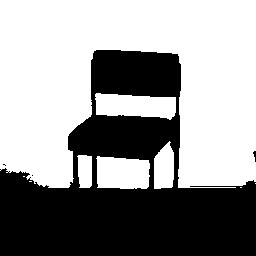
\includegraphics[width=0.15\textwidth]{img/res/e6/alg1agregadoowa1chair.jpg} &
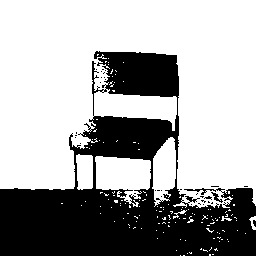
\includegraphics[width=0.15\textwidth]{img/res/e6/alg1agregadoowa2chair.jpg} &
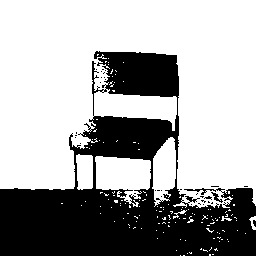
\includegraphics[width=0.15\textwidth]{img/res/e6/alg1agregadoowa3chair.jpg} \\\hline
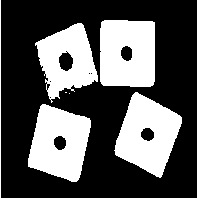
\includegraphics[width=0.15\textwidth]{img/res/e6/alg1agregadoowa1block.jpg} &
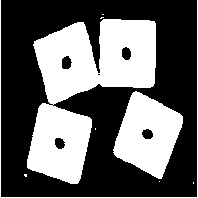
\includegraphics[width=0.15\textwidth]{img/res/e6/alg1agregadoowa2block.jpg} &
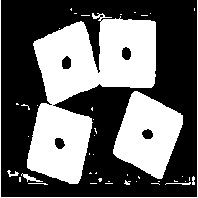
\includegraphics[width=0.15\textwidth]{img/res/e6/alg1agregadoowa3block.jpg} \\\hline
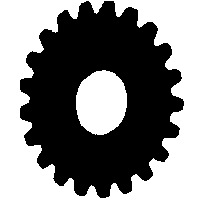
\includegraphics[width=0.15\textwidth]{img/res/e6/alg1agregadoowa102.jpg} &
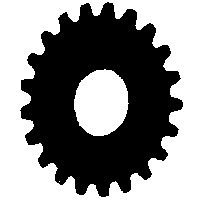
\includegraphics[width=0.15\textwidth]{img/res/e6/alg1agregadoowa202.jpg} &
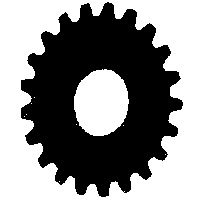
\includegraphics[width=0.15\textwidth]{img/res/e6/alg1agregadoowa302.jpg} \\\hline
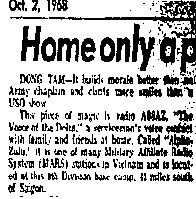
\includegraphics[width=0.15\textwidth]{img/res/e6/alg1agregadoowa109.jpg} &
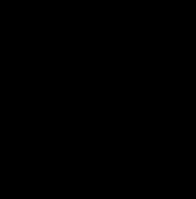
\includegraphics[width=0.15\textwidth]{img/res/e6/alg1agregadoowa209.jpg} &
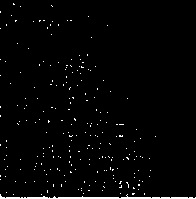
\includegraphics[width=0.15\textwidth]{img/res/e6/alg1agregadoowa309.jpg} \\\hline
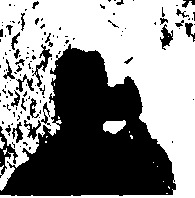
\includegraphics[width=0.15\textwidth]{img/res/e6/alg1agregadoowa107.jpg} &
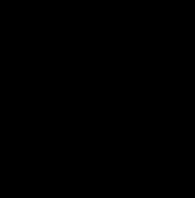
\includegraphics[width=0.15\textwidth]{img/res/e6/alg1agregadoowa207.jpg} &
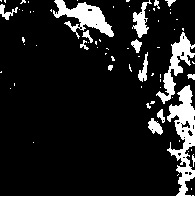
\includegraphics[width=0.15\textwidth]{img/res/e6/alg1agregadoowa307.jpg} \\\hline
\end{tabular}
\caption{Umbrales para cada imagen con la función de Dombi y diferentes $w$.\label{tab:resultexp6imagenesdombi}}
\end{table}

\begin{table}
\centering
%\resizebox*{3\textwidth}{!}{
\begin{tabular}{c||c|c|c} 
                         &\bb Media&\bb OWA (1)&\bb OWA (2)\\\hline\hline
\bb R. gausiano         &   131 &   56  &   0   \\\hline
\bb R. impulsivo 0,05   &   127 &   50  &   50  \\\hline
\bb R. impulsivo 0,2    &   136 &   50  &   50  \\\hline
\end{tabular}
\caption{Umbrales para cada imagen con la función de Dombi y diferentes $w$.\label{tab:resultexp6ruido}}
\end{table}

\begin{table}
\centering
%\resizebox*{3\textwidth}{!}{
\begin{tabular}{c|c|c} 
\multicolumn{4}{c}{}\\
\bb Media&\bb OWA (1)&\bb OWA (2)\\\hline\hline
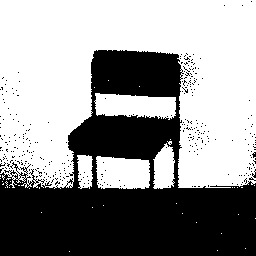
\includegraphics[width=0.15\textwidth]{img/res/e6/alg1agregadoowa1chairga.jpg} &
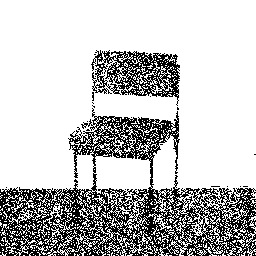
\includegraphics[width=0.15\textwidth]{img/res/e6/alg1agregadoowa2chairga.jpg} &
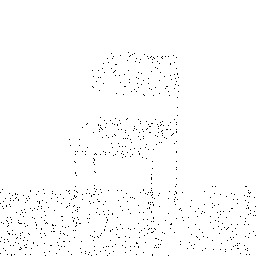
\includegraphics[width=0.15\textwidth]{img/res/e6/alg1agregadoowa3chairga.jpg} \\\hline
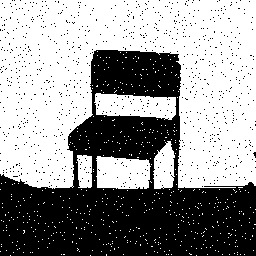
\includegraphics[width=0.15\textwidth]{img/res/e6/alg1agregadoowa1chairsp005.jpg} &
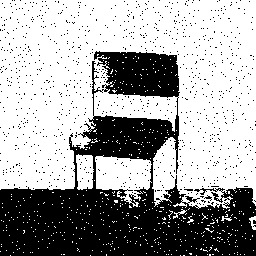
\includegraphics[width=0.15\textwidth]{img/res/e6/alg1agregadoowa2chairsp005.jpg} &
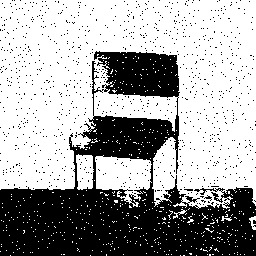
\includegraphics[width=0.15\textwidth]{img/res/e6/alg1agregadoowa3chairsp005.jpg} \\\hline
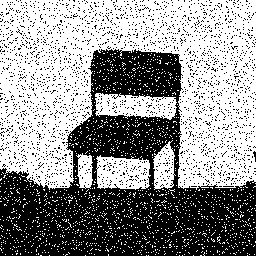
\includegraphics[width=0.15\textwidth]{img/res/e6/alg1agregadoowa1chairsp020.jpg} &
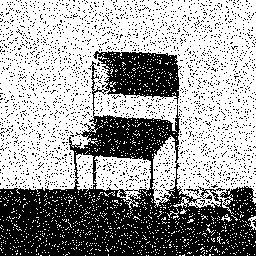
\includegraphics[width=0.15\textwidth]{img/res/e6/alg1agregadoowa2chairsp020.jpg} &
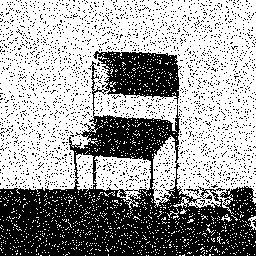
\includegraphics[width=0.15\textwidth]{img/res/e6/alg1agregadoowa3chairsp020.jpg} \\\hline
\end{tabular}
\caption{Umbrales para cada imagen con la función de Dombi y diferentes $w$.\label{tab:resultexp6imagenesruido}}
\end{table}


% EXPERIMENTO 7
\subsection{Experimento 7: sustitución de la media aritmética por funciones OWA en la construcción de los conjutos difusos para el algoritmo del umbral óptimo por similitud}

shdfkskjdhfkjshdfkjhsdkjfhkhjsdfjhsdjhfjshgfjhgsjd hsgdf hskfdhhjsd fkh sdhjfjskdfhj
\begin{table}
\centering
%\resizebox*{3\textwidth}{!}{
\begin{tabular}{c||c|c|c}
Silla                                &\bb Media&\bb OWA (1)&\bb OWA (2)\\\hline\hline
\bb Alg. 3 (a)  &   119 &   50  &   50  \\\hline
                            
\bb Alg. 3 (b)  &   103 &   114 &   172 \\\hline
\multicolumn{4}{c}{}\\
Bloques                              &\bb Media&\bb OWA (1)&\bb OWA (2)\\\hline\hline
\bb Alg. 3 (a)     &   47  &   13  &   4   \\\hline
                            
\bb Alg. 3 (b)     &   30  &   11  &   65  \\\hline
\multicolumn{4}{c}{}\\
Engranaje                            &\bb Media&\bb OWA (1)&\bb OWA (2)\\\hline\hline
\bb Alg. 3 (a)  &   84  &   4   &   1   \\\hline
                            
\bb Alg. 3 (b)  &   147 &   89  &   193 \\\hline
\multicolumn{4}{c}{}\\
Letras                               &\bb Media&\bb OWA (1)&\bb OWA (2)\\\hline\hline
\bb Alg. 3 (a)  &   200 &   255 &   236 \\\hline
                            
\bb Alg. 3 (b)  &   178 &   171 &   168 \\\hline
\multicolumn{4}{c}{}\\
Sombra                               &\bb Media&\bb OWA (1)&\bb OWA (2)\\\hline\hline
\bb Alg. 3 (a)  &   121 &   255 &   85  \\\hline
                            
\bb Alg. 3 (b)  &   101 &   136 &   136 \\\hline
\end{tabular}
\caption{Umbrales para cada imagen con la función de Dombi y diferentes $w$.\label{tab:resultexp7dombi}}
\end{table}

\begin{table}
\centering
%\resizebox*{3\textwidth}{!}{
\begin{tabular}{c||c|c|c} 
\multicolumn{4}{c}{}\\
Silla                                &\bb Media&\bb OWA (1)&\bb OWA (2)\\\hline\hline
\bb Alg. 3 (a)  &  
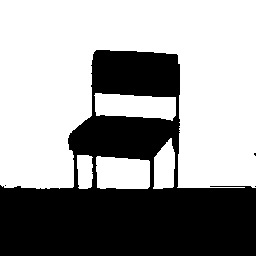
\includegraphics[width=0.12\textwidth]{img/res/e7/alg3aowa1chair.jpg} &
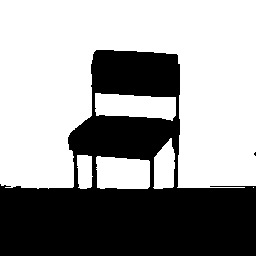
\includegraphics[width=0.12\textwidth]{img/res/e7/alg3aowa2chair.jpg} &
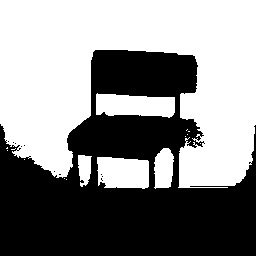
\includegraphics[width=0.12\textwidth]{img/res/e7/alg3aowa3chair.jpg} \\
\bb Alg. 3 (b)  &   
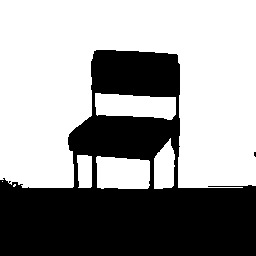
\includegraphics[width=0.12\textwidth]{img/res/e7/alg3bowa1chair.jpg} &
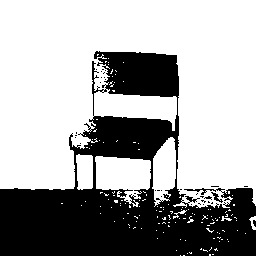
\includegraphics[width=0.12\textwidth]{img/res/e7/alg3bowa2chair.jpg} &
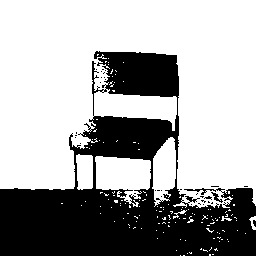
\includegraphics[width=0.12\textwidth]{img/res/e7/alg3bowa3chair.jpg} \\\hline
\multicolumn{4}{c}{}\\
Bloques                              &\bb Media&\bb OWA (1)&\bb OWA (2)\\\hline\hline
\bb Alg. 3 (a)  &  
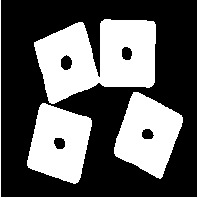
\includegraphics[width=0.12\textwidth]{img/res/e7/alg3aowa1block.jpg} &
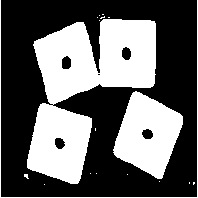
\includegraphics[width=0.12\textwidth]{img/res/e7/alg3aowa2block.jpg} &
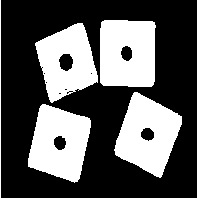
\includegraphics[width=0.12\textwidth]{img/res/e7/alg3aowa3block.jpg} \\
\bb Alg. 3 (b)  &   
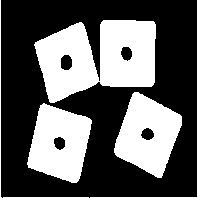
\includegraphics[width=0.12\textwidth]{img/res/e7/alg3bowa1block.jpg} &
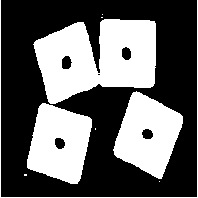
\includegraphics[width=0.12\textwidth]{img/res/e7/alg3bowa2block.jpg} &
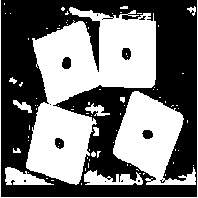
\includegraphics[width=0.12\textwidth]{img/res/e7/alg3bowa3block.jpg} \\\hline
\multicolumn{4}{c}{}\\
Engranaje                            &\bb Media&\bb OWA (1)&\bb OWA (2)\\\hline\hline
\bb Alg. 3 (a)  &  
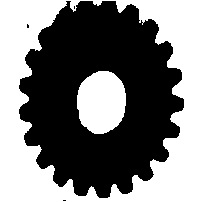
\includegraphics[width=0.12\textwidth]{img/res/e7/alg3aowa102.jpg} &
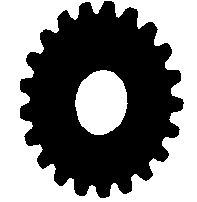
\includegraphics[width=0.12\textwidth]{img/res/e7/alg3aowa202.jpg} &
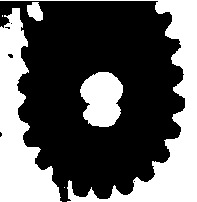
\includegraphics[width=0.12\textwidth]{img/res/e7/alg3aowa302.jpg} \\
\bb Alg. 3 (b)  &   
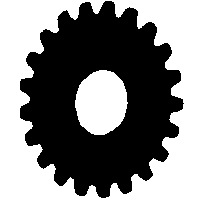
\includegraphics[width=0.12\textwidth]{img/res/e7/alg3bowa102.jpg} &
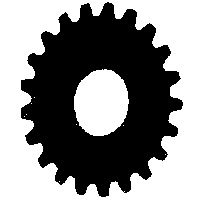
\includegraphics[width=0.12\textwidth]{img/res/e7/alg3bowa202.jpg} &
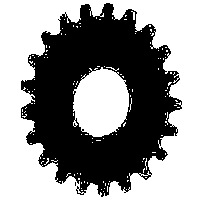
\includegraphics[width=0.12\textwidth]{img/res/e7/alg3bowa302.jpg} \\\hline
\multicolumn{4}{c}{}\\
Letras                               &\bb Media&\bb OWA (1)&\bb OWA (2)\\\hline\hline
\bb Alg. 3 (a)  &  
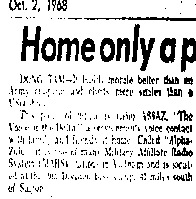
\includegraphics[width=0.12\textwidth]{img/res/e7/alg3aowa109.jpg} &
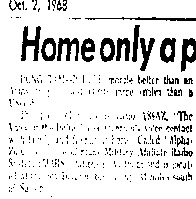
\includegraphics[width=0.12\textwidth]{img/res/e7/alg3aowa209.jpg} &
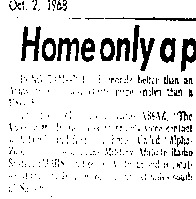
\includegraphics[width=0.12\textwidth]{img/res/e7/alg3aowa309.jpg} \\
\bb Alg. 3 (b)  &   
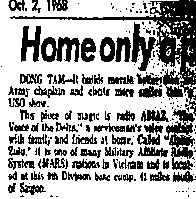
\includegraphics[width=0.12\textwidth]{img/res/e7/alg3bowa109.jpg} &
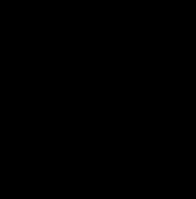
\includegraphics[width=0.12\textwidth]{img/res/e7/alg3bowa209.jpg} &
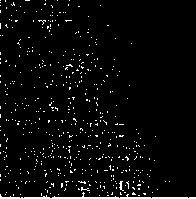
\includegraphics[width=0.12\textwidth]{img/res/e7/alg3bowa309.jpg} \\\hline
\multicolumn{4}{c}{}\\
Sombra                               &\bb Media&\bb OWA (1)&\bb OWA (2)\\\hline\hline
\bb Alg. 3 (a)  &  
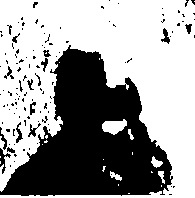
\includegraphics[width=0.12\textwidth]{img/res/e7/alg3aowa107.jpg} &
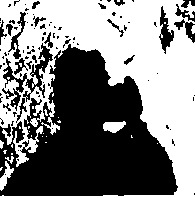
\includegraphics[width=0.12\textwidth]{img/res/e7/alg3aowa207.jpg} &
\includegraphics[width=0.12\textwidth]{img/res/e7/alg3aowa307.jpg} \\
\bb Alg. 3 (b)  &   
\includegraphics[width=0.12\textwidth]{img/res/e7/alg3bowa107.jpg} &
\includegraphics[width=0.12\textwidth]{img/res/e7/alg3bowa207.jpg} &
\includegraphics[width=0.12\textwidth]{img/res/e7/alg3bowa307.jpg} \\\hline
\end{tabular}
\caption{Umbrales para cada imagen con la función de Dombi y diferentes $w$.\label{tab:resultexp7imagenesdombi}}
\end{table}


\begin{table}
\centering
%\resizebox*{3\textwidth}{!}{
\begin{tabular}{c||c|c|c}
R. gausiano                         &\bb Media&\bb OWA (1)&\bb OWA (2)\\\hline\hline
\bb Alg. 3 (a)  &   132 &   56  &   0   \\\hline
                            
\bb Alg. 3 (b)  &   99  &   154 &   159 \\\hline
\multicolumn{4}{c}{}\\
R. impulsivo 0,05                    &\bb Media&\bb OWA (1)&\bb OWA (2)\\\hline\hline
\bb Alg. 3 (a)  &   144 &   50  &   50  \\\hline
                            
\bb Alg. 3 (b)  &   111 &   122 &   172 \\\hline
\multicolumn{4}{c}{}\\
R. impulsivo 0,2                     &\bb Media&\bb OWA (1)&\bb OWA (2)\\\hline\hline
\bb Alg. 3 (a)     &   152 &   50  &   0   \\\hline
                            
\bb Alg. 3 (b)     &   127 &   131 &   172 \\\hline
\end{tabular}
\caption{Umbrales para cada imagen con la función de Dombi y diferentes $w$.\label{tab:resultexp7ruido}}
\end{table}

\begin{table}
\centering
%\resizebox*{3\textwidth}{!}{
\begin{tabular}{c||c|c|c} 
\multicolumn{4}{c}{}\\
Silla                                &\bb Media&\bb OWA (1)&\bb OWA (2)\\\hline\hline
\bb Alg. 3 (a)  &  
\includegraphics[width=0.12\textwidth]{img/res/e7/alg3aowa1chairga.jpg} &
\includegraphics[width=0.12\textwidth]{img/res/e7/alg3aowa2chairga.jpg} &
\includegraphics[width=0.12\textwidth]{img/res/e7/alg3aowa3chairga.jpg} \\
\bb Alg. 3 (b)  &   
\includegraphics[width=0.12\textwidth]{img/res/e7/alg3bowa1chairga.jpg} &
\includegraphics[width=0.12\textwidth]{img/res/e7/alg3bowa2chairga.jpg} &
\includegraphics[width=0.12\textwidth]{img/res/e7/alg3bowa3chairga.jpg} \\\hline
\multicolumn{4}{c}{}\\
Bloques                              &\bb Media&\bb OWA (1)&\bb OWA (2)\\\hline\hline 
\bb Alg. 3 (a)  &  
\includegraphics[width=0.12\textwidth]{img/res/e7/alg3aowa1chairsp005.jpg} &
\includegraphics[width=0.12\textwidth]{img/res/e7/alg3aowa2chairsp005.jpg} &
\includegraphics[width=0.12\textwidth]{img/res/e7/alg3aowa3chairsp005.jpg} \\
\bb Alg. 3 (b)  &   
\includegraphics[width=0.12\textwidth]{img/res/e7/alg3bowa1chairsp005.jpg} &
\includegraphics[width=0.12\textwidth]{img/res/e7/alg3bowa2chairsp005.jpg} &
\includegraphics[width=0.12\textwidth]{img/res/e7/alg3bowa3chairsp005.jpg} \\\hline
\multicolumn{4}{c}{}\\
Engranaje                            &\bb Media&\bb OWA (1)&\bb OWA (2)\\\hline\hline
\bb Alg. 3 (a)  &  
\includegraphics[width=0.12\textwidth]{img/res/e7/alg3aowa1chairsp020.jpg} &
\includegraphics[width=0.12\textwidth]{img/res/e7/alg3aowa2chairsp020.jpg} &
\includegraphics[width=0.12\textwidth]{img/res/e7/alg3aowa3chairsp020.jpg} \\
\bb Alg. 3 (b)  &   
\includegraphics[width=0.12\textwidth]{img/res/e7/alg3bowa1chairsp020.jpg} &
\includegraphics[width=0.12\textwidth]{img/res/e7/alg3bowa2chairsp020.jpg} &
\includegraphics[width=0.12\textwidth]{img/res/e7/alg3bowa3chairsp020.jpg} \\\hline
\end{tabular}
\caption{Umbrales para cada imagen con la función de Dombi y diferentes $w$.\label{tab:resultexp7imagenesdombi}}
\end{table}

